\begin{scanpage}{0091}{74}
source [5, 37]. In this case it is sufficient to consider only the nonuniform part of the current which is caused by the discontinuity of the surface, and we will do this in this Chapter. The equations obtained in this way are generalized to the case when the observation direction does not coincide with the direction of the source.
\sectiontitle{13}{The Physical Optics Approach}
Let us investigate the diffraction of plane electromagnetic wave
\[\mathbf E=\mathbf E_0e^{ik(y\sin\gamma+z\cos\gamma)}\tag{13.01}\]
on a finite, ideally conducting cylinder of radius $a$ and length $l$. Let us position the spherical coordinate system in such a way that its origin is at the center of the cylinder, and the normal $\mathbf n$ to the incident wave front lies in the half-plane $\varphi=\frac\pi2$ and forms an angle $\gamma$ $(0<\gamma<\frac\pi2)$ with the $z$ axis (Figure 24).

\noindent\begin{minipage}{.46\linewidth}\centering
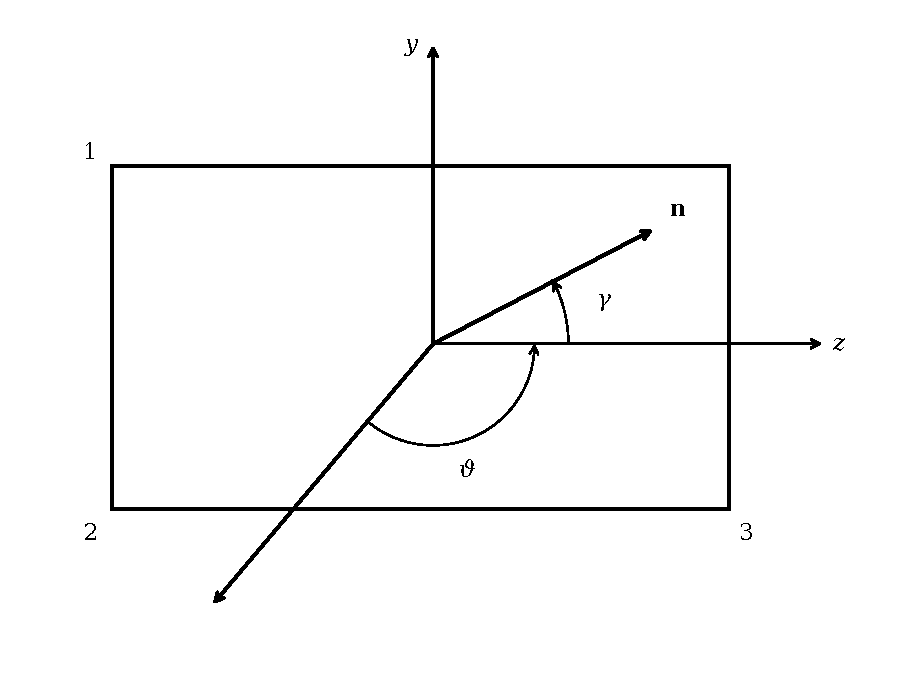
\includegraphics[width=.9\linewidth]{images/recreated/b-0091-fig24.pdf}

Figure 24. Diffraction of a plane wave by a finite cylinder. $\mathbf n$ is the normal to the incident wave front.
\end{minipage}\hfill\begin{minipage}{.50\linewidth}
An incident wave having an arbitrary linear polarization always may be represented as the sum of two waves with mutually perpendicular polarizations. Therefore, for a complete solution of the problem, it is sufficient to investigate two particular cases of incident wave polarization:
\end{minipage}\par\medskip

(1) E-polarization, when the incident wave electric vector is perpendicular to the plane $(\mathbf E_0\perp yoz)$ and

(2) H-polarization, when $\mathbf H_0\perp yoz$.

The uniform part of the current excited on the cylindrical surface by wave (13.01) has, with the E-polarization, the components:
\end{scanpage}
